\chapter{Appendix: Faster Whisper and Transcription Models}
\label{appendix-faster-whisper}

This appendix explores Faster Whisper, an optimized implementation of OpenAI's Whisper model for speech-to-text transcription and translation. It analyzes its main features, architecture, and compares performance among the different available models.

\section{Main Features}
\label{sec:faster-whisper-features}

Faster Whisper represents a significant improvement over the original Whisper implementation, standing out for:

\begin{itemize}
	\item \textbf{CTranslate2 Optimization}: Uses the CTranslate2 toolkit to optimize model inference.
	\item \textbf{Lower Memory Consumption}: Significantly reduces memory usage through quantization techniques.
	\item \textbf{Hardware Acceleration}: Efficiently leverages CPU and GPU through parallelization.
	\item \textbf{Voice Detection}: Integrates VAD (Voice Activity Detection) to improve accuracy.
\end{itemize}

\section{System Architecture}
\label{sec:faster-whisper-architecture}

\begin{figure}[H]
	\label{fig:whisper}
	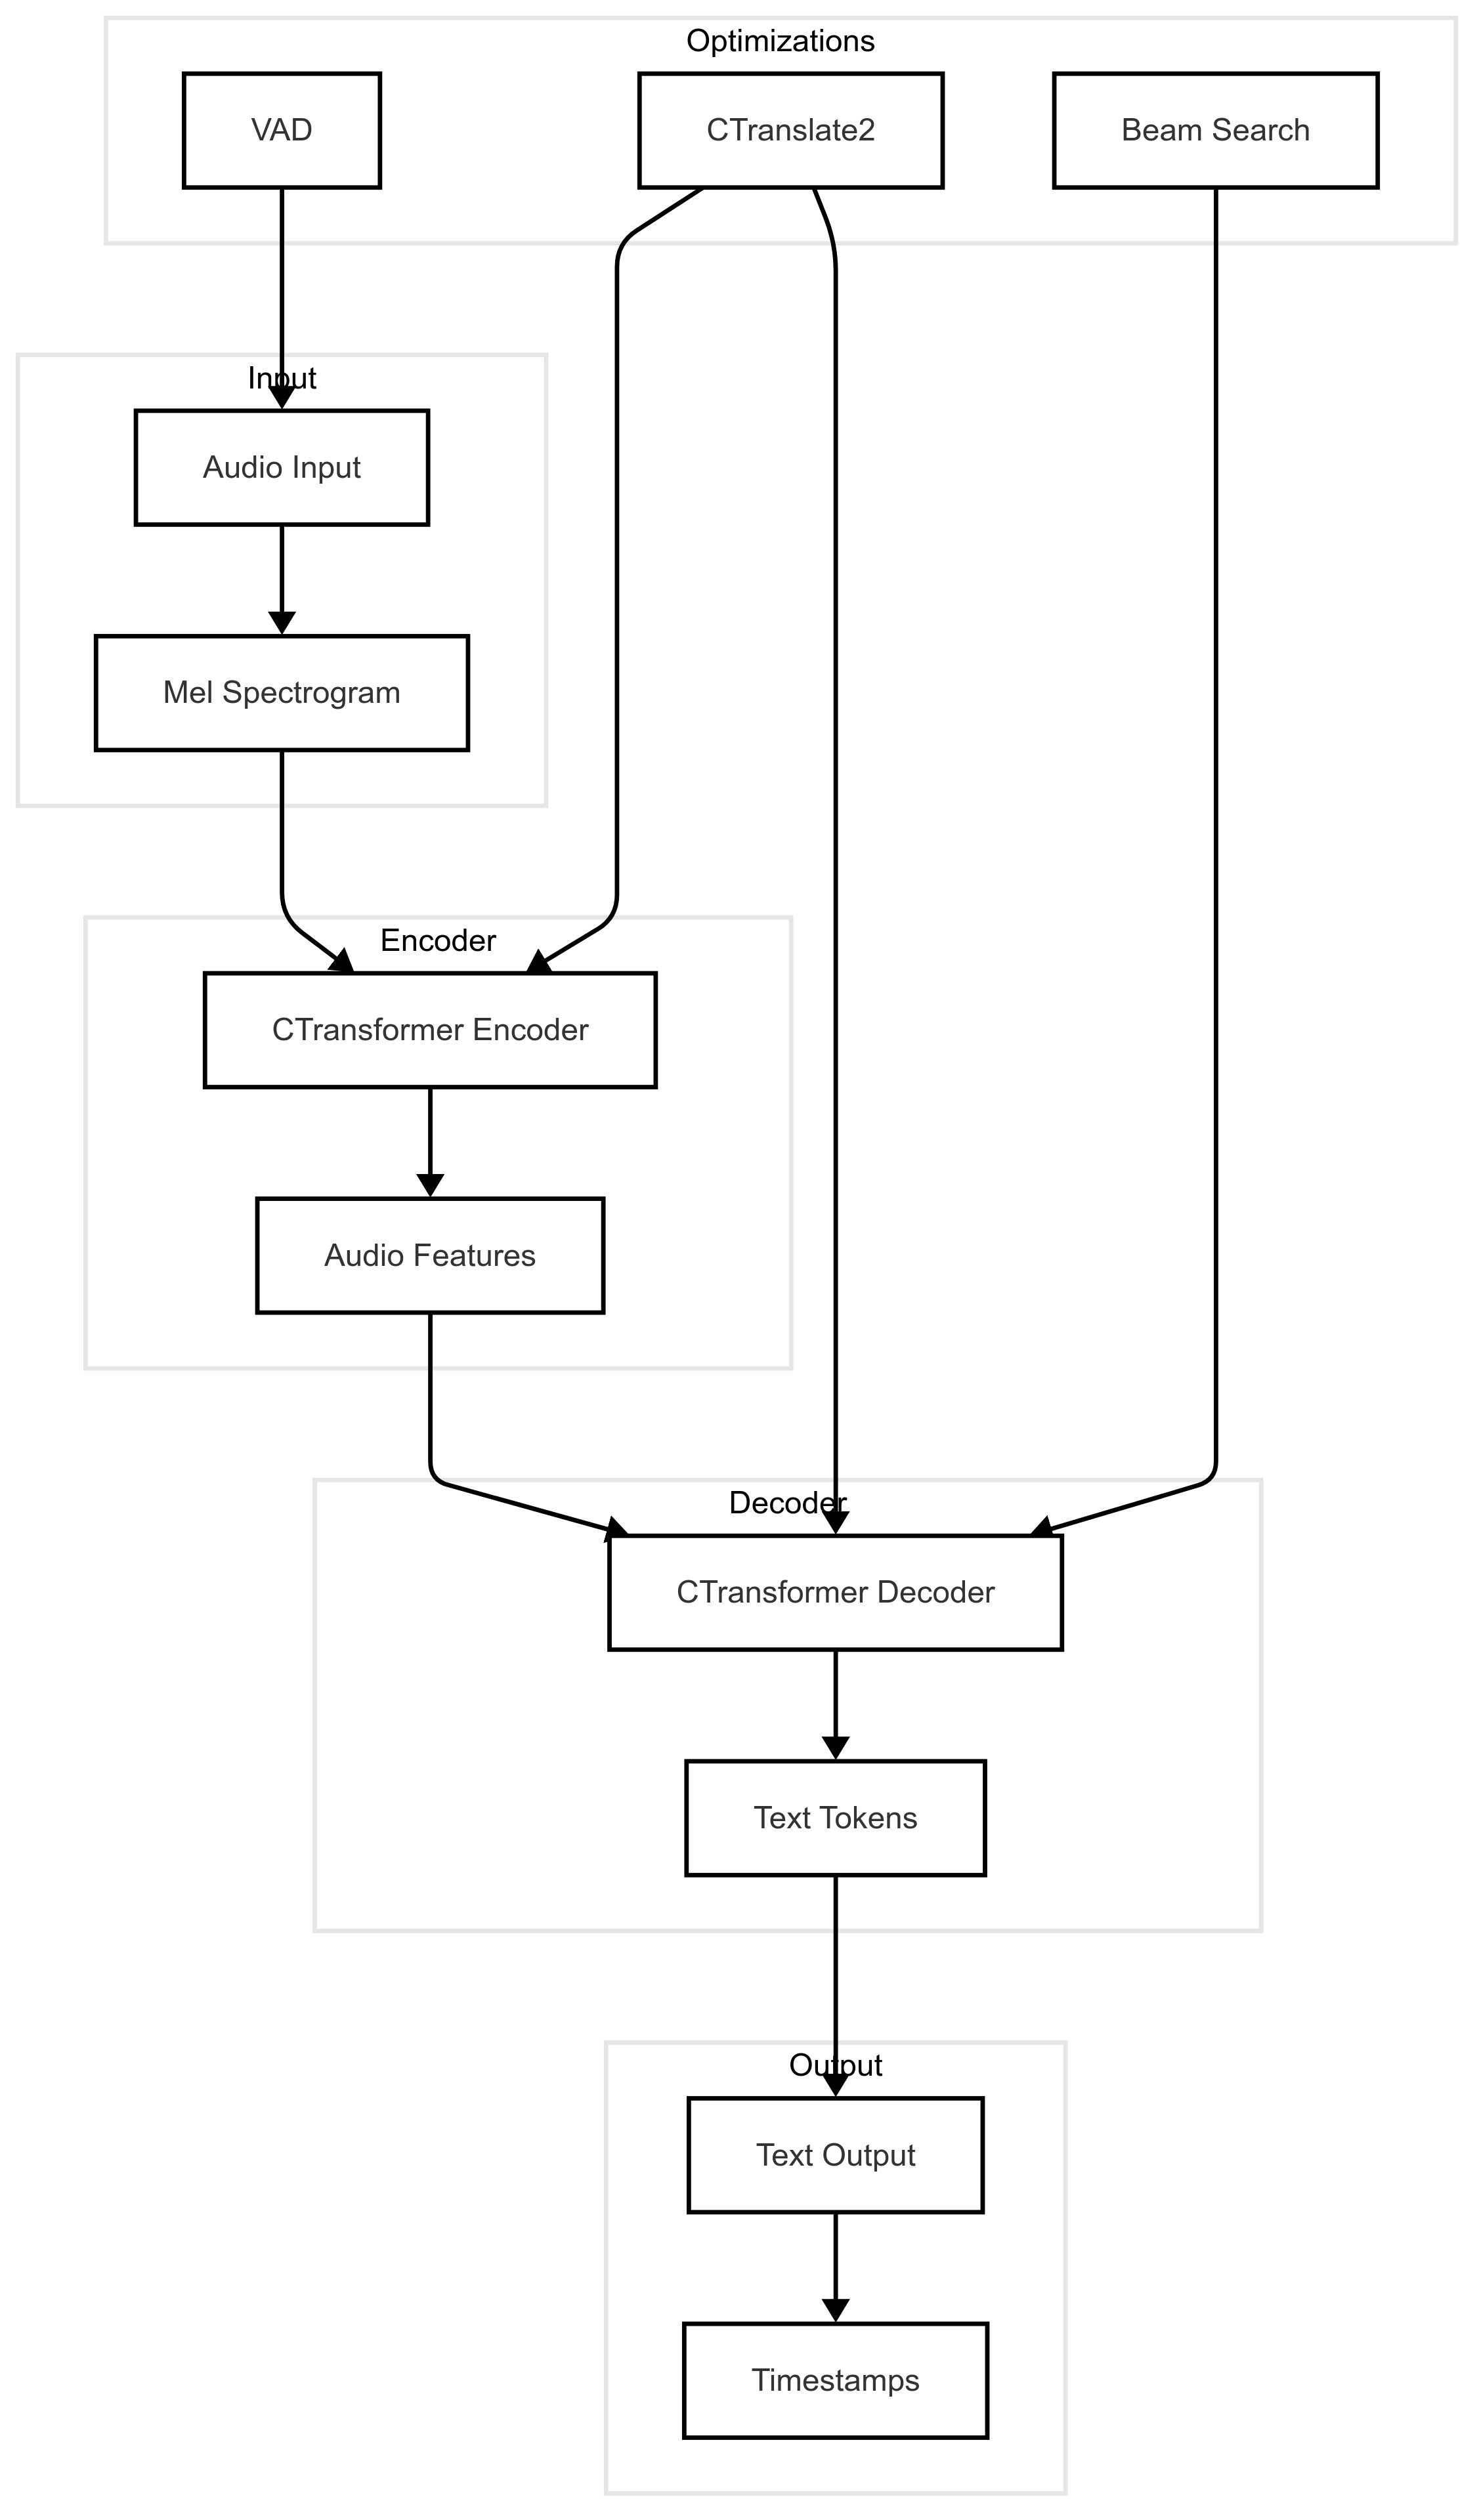
\includegraphics[width=0.8\textwidth]{figuras/whisper.png}
	\caption{Faster Whisper Architecture}
\end{figure}

The Faster Whisper architecture consists of several specialized modules working together to provide efficient transcription:

\subsection{Main Components}
\label{subsec:main-components}

\subsubsection{Audio Preprocessing}
The system processes audio input through:
\begin{equation}
	\text{mel} = \text{log}(\max(\text{STFT}(x), \epsilon))
\end{equation}
where STFT is the Short-Time Fourier Transform and $\epsilon$ is a small value for numerical stability.

\subsubsection{CTransformer}
The implementation uses CTranslate2 to optimize:
\begin{itemize}
	\item \textbf{Encoder}: Processes the mel spectrogram into audio representations.
	\item \textbf{Decoder}: Generates text tokens through cross-attention.
\end{itemize}

\section{Whisper Models Comparison}
\label{sec:whisper-models-comparison}

\begin{table}[H]
	\label{tab:whisper-models}
	\begin{tabular}{|p{2cm}|p{2cm}|p{3cm}|p{3cm}|p{3cm}|}
		\hline
		\textbf{Model} & \textbf{Parameters} & \textbf{RAM (FP16)} & \textbf{WER} & \textbf{Relative Speed} \\
		\hline
		Tiny            & 39M                 & 1GB                 & 7.1\%        & 32x                         \\
		\hline
		Base            & 74M                 & 1.5GB               & 6.1\%        & 16x                         \\
		\hline
		Small           & 244M                & 2.5GB               & 5.2\%        & 8x                          \\
		\hline
		Medium          & 769M                & 4.5GB               & 4.3\%        & 4x                          \\
		\hline
		Large           & 1550M               & 7.5GB               & 3.6\%        & 1x                          \\
		\hline
	\end{tabular}
	\caption{Whisper models comparison}
\end{table}

\subsection{Features by Model}
\label{subsec:model-features}

\begin{itemize}
	\item \textbf{Tiny}:
	      \begin{itemize}
		      \item Ideal for devices with limited resources
		      \item Best option for real-time transcription
		      \item Acceptable performance in clean audio conditions
	      \end{itemize}

	\item \textbf{Base}:
	      \begin{itemize}
		      \item Balance between performance and resources
		      \item Suitable for web applications
		      \item Good performance across multiple languages
	      \end{itemize}

	\item \textbf{Small}:
	      \begin{itemize}
		      \item Significant accuracy improvement over Base
		      \item Robust support for multiple accents
		      \item Reliable detection of language changes
	      \end{itemize}

	\item \textbf{Medium}:
	      \begin{itemize}
		      \item High accuracy in challenging conditions
		      \item Excellent performance with noisy audio
		      \item Advanced punctuation capabilities
	      \end{itemize}

	\item \textbf{Large}:
	      \begin{itemize}
		      \item Maximum available accuracy
		      \item Best performance on complex audio
		      \item Superior translation capability
	      \end{itemize}
\end{itemize}

\section{Optimizations}
\label{sec:optimizations}

\subsection{Quantization Techniques}
\label{subsec:quantization}

Faster Whisper implements several quantization techniques:

\begin{itemize}
	\item \textbf{INT8}: Reduces model size by 4x with minimal accuracy loss
	\item \textbf{INT16}: Balance between accuracy and size
	\item \textbf{FLOAT16}: Maximum accuracy with reduced memory
\end{itemize}

\subsection{Parallelization}
\label{subsec:parallelization}

The system implements multiple levels of parallelization:

\begin{itemize}
	\item \textbf{Batch Processing}: Processes multiple segments simultaneously
	\item \textbf{Thread Pooling}: Optimizes CPU utilization
	\item \textbf{GPU Acceleration}: Leverages CUDA for parallel processing
\end{itemize}

\section{Implementation Considerations}
\label{sec:implementation-considerations}

\subsection{Model Selection}
Model choice should consider:

\begin{itemize}
	\item \textbf{Available Resources}: Memory and processing capacity
	\item \textbf{Latency Requirements}: Necessary response time
	\item \textbf{Required Accuracy}: Error tolerance
\end{itemize}

\subsection{Deployment Strategies}
Deployment considerations:

\begin{itemize}
	\item \textbf{Edge Computing}: On-device processing for lower latency
	\item \textbf{Server-Side}: Greater processing capacity but higher latency
	\item \textbf{Hybrid}: Combination according to specific needs
\end{itemize}

\chapter{Appendix: Kokoro TTS}
\label{appendix-kokoro}

This appendix explores Kokoro TTS, an open-source speech synthesis model that stands out for its efficiency and quality comparable to larger models, despite having only 82 million parameters. The model implements a lightweight architecture based on StyleTTS 2 and ISTFTNet, designed to deliver high-quality speech synthesis with limited computational resources.

\section{System Architecture}
\label{sec:kokoro-architecture}

The Kokoro TTS architecture is based on two main components: StyleTTS 2 and ISTFTNet. This combination enables efficient speech synthesis while maintaining high output quality.

\subsection{Main Components}
\label{subsec:kokoro-main-components}

\begin{itemize}
	\item \textbf{Misaki G2P}: Grapheme-to-phoneme conversion system that supports multiple languages.
	\item \textbf{Style Encoder}: Encodes voice style characteristics from reference audio.
	\item \textbf{Decoder}: Generates acoustic features based on phonemes and style.
	\item \textbf{ISTFT Network}: Performs final audio synthesis through inverse Fourier transform.
\end{itemize}

\section{Technical Features}
\label{sec:technical-features}

\subsection{Model Specifications}
\begin{itemize}
	\item \textbf{Parameters}: 82 million
	\item \textbf{Base Architecture}: StyleTTS 2 + ISTFTNet
	\item \textbf{License}: Apache 2.0
	\item \textbf{Audio Format}: 24kHz, mono
\end{itemize}

\subsection{Dataset}
Training was conducted exclusively with permissible audio data:
\begin{itemize}
	\item Public domain audio
	\item Audio with permissive licenses (Apache, MIT)
	\item Synthetic audio from commercial models
\end{itemize}

\section{Voice Analysis}
\label{sec:voice-analysis}

\subsection{Grading System}
\label{subsec:grading-system}

The system evaluates voices using two main metrics:

\begin{itemize}
	\item \textbf{Objective Quality}:
	      \begin{itemize}
		      \item A: Exceptional quality
		      \item B: Good quality
		      \item C: Acceptable quality
		      \item D: Limited quality
	      \end{itemize}

	\item \textbf{Training Duration}:
	      \begin{itemize}
		      \item HH: 10-100 hours
		      \item H: 1-10 hours
		      \item MM: 10-100 minutes
		      \item M: 1-10 minutes
	      \end{itemize}
\end{itemize}

\subsection{Voice Distribution}
\label{subsec:voice-distribution}

\begin{table}[H]
	\centering
	\label{tab:voice-distribution}
	\begin{tabular}{|l|c|c|c|l|}
		\hline
		\textbf{Language}  & \textbf{F} & \textbf{M} & \textbf{Total} & \textbf{Average Quality} \\
		\hline
		American English & 11         & 9          & 20             & B-                     \\
		\hline
		British English & 4          & 4          & 8              & C+                     \\
		\hline
		Japanese          & 4          & 1          & 5              & C+                     \\
		\hline
		Mandarin Chinese   & 4          & 4          & 8              & D+                     \\
		\hline
		Spanish          & 1          & 2          & 3              & C                      \\
		\hline
		French          & 1          & 0          & 1              & B-                     \\
		\hline
		Hindi            & 2          & 2          & 4              & C                      \\
		\hline
		Italian         & 1          & 1          & 2              & C                      \\
		\hline
		Brazilian Portuguese     & 1          & 2          & 3              & C                      \\
		\hline
	\end{tabular}
	\caption{Voice distribution and quality by language}
\end{table}

\section{Performance and Limitations}
\label{sec:performance}

\subsection{Optimal Operating Ranges}
\label{subsec:optimal-ranges}

Model performance varies according to text length:
\begin{itemize}
	\item \textbf{Optimal Range}: 100-200 tokens
	\item \textbf{Reduced Performance}: <20 tokens
	\item \textbf{Possible Acceleration}: >400 tokens
\end{itemize}

\subsection{Training Costs}
\label{subsec:training-costs}

Kokoro's training has been remarkably efficient:
\begin{itemize}
	\item \textbf{GPU Hours}: 1000 hours on A100 80GB
	\item \textbf{Total Cost}: Approximately \$1000 USD
	\item \textbf{Average Rate}: \$1/hour
\end{itemize}

\section{Comparison with Other Models}
\label{sec:model-comparison}

\begin{table}[H]
	\centering
	\label{tab:model-comparison}
	\begin{tabular}{|l|c|c|c|c|}
		\hline
		\textbf{Model} & \textbf{Parameters} & \textbf{Voices} & \textbf{Languages} & \textbf{License} \\
		\hline
		Kokoro          & 82M                 & 54             & 8                & Apache            \\
		\hline
		Coqui           & 1000M               & 1087           & 100+             & MIT               \\
		\hline
		Bark            & 900M                & 100+           & 100+             & MIT               \\
		\hline
	\end{tabular}
	\caption{Comparison with similar TTS models}
\end{table}